\documentclass[pdftex,english,11pt,parskip=half]{scrartcl}
\usepackage{palatino}
\usepackage{mathpazo}
\usepackage[margin=0.7in]{geometry}
%\usepackage{parskip}
\usepackage[compact]{titlesec}
\usepackage{amsmath,amssymb}
\usepackage{graphicx}
\usepackage{babel}
\usepackage{framed}
\usepackage{wrapfig}
\usepackage{subfig}
\usepackage[labelfont=bf,font=small,format=plain]{caption}
\usepackage{doi}
\usepackage{booktabs}
\usepackage{longtable}
\usepackage{multirow}
\usepackage[table]{xcolor}
\usepackage{wrapfig}
\usepackage{colortbl}
\usepackage{pdflscape}
\usepackage{tabu}
\usepackage{threeparttable}
\usepackage{threeparttablex}
\usepackage{array}
\usepackage[normalem]{ulem}
\usepackage{makecell}
\usepackage{float}
%\usepackage[authoryear]{natbib}
\usepackage[numbers]{natbib}
\usepackage{url,hyperref,color}
\definecolor{darkblue}{rgb}{0.0,0.0,0.75}
\hypersetup{colorlinks,breaklinks,
            linkcolor=darkblue,urlcolor=darkblue,
            anchorcolor=darkblue,citecolor=darkblue}
\newcommand{\fixme}[1]{{\color{red} #1}}
\renewcommand\thesection{\Alph{section}}
\renewcommand{\familydefault}{\sfdefault}
\newcommand{\tabitem}{~~\llap{\textbullet}~~}
\begin{document}
\addtokomafont{section}{\large}
\def\bf{\normalfont\bfseries}
\pagestyle{empty}

\section*{Research Education Program Plan}

\section{Significance}
\vspace{-0.1in}

\begin{quotation}
``Does the proposed program address a key audience and an important aspect or important need in training in rigor and reproducibility? Is there convincing evidence in the application that the proposed program will significantly advance the stated goal of the program?"
\end{quotation}

\section{Innovation}
\vspace{-0.1in}

\begin{quotation}
``Taking into consideration the nature of the proposed research education program, does the applicant make a strong case for this program effectively reaching an audience in need of the program's offerings? Where appropriate, is the proposed program developing or utilizing innovative approaches and latest best practices to improve the knowledge and/or skills of the intended audience?"
\end{quotation}

These modules will teach the principals of reproducibility as well as introduce researchers to tools for implementing reproducible research workflows. The implementation portion of these modules will focus on tools from the open-source R programming language. R can be freely, quickly, and easily downloaded and installed to a user's computer, allowing new users to get started quickly, a critical consideration for usable scientific software \cite{list2017ten}. R has been maintained for over a decade by the R Development Core Team and works with all major computing platforms, ensuring  widespread access, stability, and compatability, also critical for ease-of-use \cite{baumer2017lessons, altschul2013anatomy}. R offers a well-developed environment for creating new tools that extend the core language \cite{wickham2015r} and includes ample tools for documenting research workflows \cite{xie2015dynamic, xie2016bookdown}. R's status as the \textit{lingua franca} of statisticians and biostatisticians means that its use in early stages of experimental data recording and pre-processing can help foster closer collaborations between laboratory-based scientists and statisticians throughout the research process. R can be scaled as the volume of data in projects grows \cite{list2017ten}, as it includes tools to interface with distributed computing platforms (e.g., \textit{Hadoop} \cite{pathak2014rhadoop}, \textit{Spark} \cite{sparklyr}), and its scripts can be integrated within workflow management systems (e.g., \textit{Galaxy} \cite{goecks2010galaxy, walker2016models}). 

\section{Approach}

\begin{quotation}
``Does the proposed program clearly state its goals and objectives, including the audience to be reached, the content to be conveyed, and the intended outcome?  Is there evidence that the program is based on a sound rationale, as well as sound educational concepts and principles? Is the plan for evaluation sound and likely to provide information on the effectiveness of the program?"
\end{quotation}

\subsection{Proposed Research Education Program Plan}

\begin{quotation}
``While the proposed research education program may complement ongoing research training and education occurring at the applicant institution, the proposed educational experiences must be distinct from those research training and research education programs currently receiving federal support. When research training programs are on-going in the same department, the applicant organization should clearly distinguish between the activities in the proposed research education program and the research training supported by the training program. The research education proposed must be \textbf{targeted to trainees and investigators at any level}. State the \textbf{goals for education} and \textbf{justify the area of training} selected for module development in terms of its \textbf{relevance and potential impact} on improving the development of skills and knowledge important for conducting rigorous and reproducible research. Describe the \textbf{subject material} to be covered.  Describe the \textbf{format} for the training module proposed and \textbf{justify it in terms of the education goals}.  The \textbf{length} of the proposed training module should be explained in terms of \textbf{scope and depth of coverage} of the subject matter.  In addition, \textbf{how the research education will be utilized by trainees or investigators} should be described---for example, a module on how to avoid confirmation bias to be taken by all beginning laboratory workers, or a module on appropriate design of animal studies to be taken immediately prior to beginning such work.  Describe the \textbf{plans for piloting and evaluating the effectiveness} of the training module. Describe \textbf{plans for making the proposed training module section 508 compliant of the Rehabilitation Act} (29 U.S.C. '794 d), as amended by the Workforce Investment Act of 1998 (P.L. 105 – 220; see http://www.section508.gov/ for additional information). Provide a \textbf{timeline for module development, piloting and refinement, dissemination, evaluation, and maintenance}.  This timeline must propose \textbf{making the training publicly available within two years} of the award date."
\end{quotation}

\subsubsection{Educational goals of the modules}

The importance of computational reproducibility of scientific research is increasingly recognized by scientists, journals, and funding agencies, with such ``computationally reproducible" research requiring that all data and code for a research project be available and that this data and code can be used to regenerate study findings either by the original researcher or by other researchers \cite{ellis2017share, ram2013git}.

Every extra step of data formatting is another chance to introduce an error in the data. Therefore, by keeping research data pipelines simple---which can be more easily achieved if data is initially recorded in a format amenable to later data pre-processing, analysis, and visualization---researchers can decrease the potential for errors in the data and therefore improve the rigor and reproducibility of their research.

\textbf{Improving the Reproducibility of Experimental Data Recording} One key concept for improving the reproducibility of experimental data collection is understanding how to create and use the ``tidy" data format, which enables later data analysis using R's \textit{tidyverse} framework. The \textit{tidyverse} framework enables powerful and user-friendly data management, processing, and analysis by combining simple tools to solve complex, multi-step problems, and this framework is enabled by ensuring those simple tools share a common interface: a ``tidy" data format \cite{ross2017declutter, silge2016tidytext, wickham2016ggplot2, wickham2016r}. Working within the R framework facilitates research that adheres to standards of reproducibility through scriptable data analysis that can easily be placed under version control \cite{bryan2017excuse}. Since the tools are simple and share a common interface, they are easier to learn, use, and combine than tools created in the classical R framework \cite{ross2017declutter, lowndes2017our, reviewer2017review, mcnamara2016state}. This \textit{tidyverse} framework is quickly becoming the standard taught in introductory R courses and books \cite{hicks2017guide, baumer2015data, kaplan2017teaching, stander2017enthusing, reviewer2017review, mcnamara2016state} (see also Letters of Support [LOS], Kimmel, Peng), ensuring ample training resources for researchers new to programming, including books (e.g., \cite{baumer2017modern, lifesciencesR}, some freely available online, e.g., \cite{wickham2016r}), massive open online courses (MOOCs), onsite university courses \cite{baumer2015data, kaplan2017teaching, stander2017enthusing}, and Software Carpentry workshops \cite{wilson2014software, pawlik2017developing}. Further, tools that extend the tidyverse have been created to enable high-quality data analysis and visualization in several domains, including text mining \cite{silge2017text}, microbiome studies \cite{mcmurdie2013phyloseq}, natural language processing \cite{RJ-2017-035}, network analysis \cite{RJ-2017-023}, ecology \cite{hsieh2016inext}, and genomics \cite{yin2012ggbio}.

RStudio allows users to create their own custom ``Project" template, suited to a specific type of data analysis or software development, which can then be registered and accessed by other users \cite{rstudioprojecttemplate}. While a ``Project" can have any internal structure, a common structure can be enforced for a certain type of project through the creation of a new ``Project" template, which defines the required subdirectories, structure, and file names of common elements that must exist in the project \cite{rstudioprojecttemplate}. This template, when selected by a future user, will create a new directory with a ``skeleton" structure, potentially including templated files (e.g., for metadata). Projects saved in this format can be easily put under \textit{Git} version control in \textit{RStudio}, which includes a pane that allows users to work under version control without learning command-line version control language and, if desired, easily connect the project with an online version of the project hosted on \textit{GitHub}. This ``project" framework has recently been encouraged by a number of researchers as a way to enable computationally reproducible research, especially for research conducted by teams \cite{marwick2017packaging, parker2017opinionated, lowndes2017our}, and the use of \textit{Git} and \textit{GitHub} has also been encouraged as a tool to enable reproducible research \cite{piccolo2016tools, ram2013git, bryan2017excuse, lowndes2017our, cetinkaya2017infrastructure}.  

\textbf{Improving the Reproducibility of Experimental Data Pre-Processing.} Scriptable software tools bring key advantages compared to GUI software in terms of data pre-processing \cite{cetinkaya2017infrastructure, huber2015orchestrating, preeyanon2014reproducible, piccolo2016tools}, but it is critical to provide some training on the use of these tools for researchers new to programming. Expertise with a scripting language is not universal across the biomedical community, although literacy in programming is increasing in the sciences \cite{ram2013git}, and many now recommend programming as a critical skill for all biology Ph.D. students \cite{list2017ten}. 

\textit{Contrast the lack of guidance on experimental data recording for academic research with the guidelines from industry, including ``Good laboratory practice").}

\subsubsection{Module subject material}

We propose to develop two collections of modules, \textbf{Improving the Reproducibility of Experimental Data Recording} and \textbf{Improving the Reproducibility of Experimental Data Pre-Processing}. 


\begin{landscape}\begingroup\fontsize{9}{11}\selectfont
\rowcolors{2}{white}{gray!6}

\begin{longtable}[t]{>{\bfseries\raggedright\arraybackslash}p{10em}>{\raggedright\arraybackslash}p{30em}>{\raggedright\arraybackslash}p{15em}>{\raggedright\arraybackslash}p{3em}>{\raggedright\arraybackslash}p{15em}}
\caption{\label{tab:}Modules for the first sequence, \textbf{'Improving the Reproducibility of Experimental Data Recording'}. The color of each module's title indicates whether the module focuses on \textbf{Principles} (blue), \textbf{Implementation} (red), or \textbf{Case study examples} (black). This table is continued over several pages.}\\
\hiderowcolors
\toprule
Module title & Description of module content & Objectives (After taking the module, the trainee can ...) & Video length & Extra educational materials\\
\midrule
\endfirsthead
\caption[]{Modules for the first sequence, \textbf{'Improving the Reproducibility of Experimental Data Recording'}. The color of each module's title indicates whether the module focuses on \textbf{Principles} (blue), \textbf{Implementation} (red), or \textbf{Case study examples} (black). This table is continued over several pages. \textit{(continued)}}\\
\toprule
Module title & Description of module content & Objectives (After taking the module, the trainee can ...) & Video length & Extra educational materials\\
\midrule
\endhead
\
\endfoot
\bottomrule
\endlastfoot
\showrowcolors
\textcolor{blue}{\textbf{Separating data recording and analysis}} & Many biomedical laboratories currently use spreadsheets, with embedded macros, 
      to both record and analyze experimental data. This practice empedes the transparency
      and reproducibility of both data recording and data analysis. In this module, we 
      will describe this common practice and explain how it impedes the transparency and
      reproducibility of data recording and analysis. We will then outline alternative
      approaches that separate the steps of data recording and data analysis and explain
      how these alternative approaches can improve the reproducbility of biomedical 
      research. & \tabitem Explain the difference between data recording and data analysis 

     \tabitem Understand why collecting data on spreadsheets with embedded macros
        impedes transparency and reproducibility 

      \tabitem List alternative approaches that separate data recording and data analysis to 
        improve transparency and reproducibility & 15 & \tabitem Discussion questions about data recording approaches the trainee has 
      previously used in research projects and the benefits
      and limitations of those approaches in terms of data transparency and 
      reproducibility 

    \tabitem Short audio recording of two Co-Is giving their
      own answers to these discussion questions\\
\textcolor{blue}{\textbf{Principles and power of structured data formats}} & The format in which experimental data is recorded can have a large influence
      on how easy and likely it is to implement reproducibility tools in later stages of
      data pre-processing, analysis, and visualization. Recording data in a 'structured'
      format brings many benefits for later stages of the research process, 
      especially in terms of improving reproducibility.
      In this module, we will explain what makes a dataset 'structured' and
      why this format is a powerful tool for reproducible research. & \tabitem List the characteristics of a structured data format 

      \tabitem Describe how using a structured data format when recording experimental 
      data can improve the transparency and reproducibility of research

      \tabitem Outline other benefits of using a structured format when recording data & 10 & \tabitem Applied exercise: For example datasets, specify whether each is in a 
      structured data format and, in cases where it is not, draft a structured
      format that could be used to record the data 

    \tabitem Video walking trainees 
      through solutions to the applied exercise\\
\textcolor{red}{\textbf{The 'tidy' data format: an implementation of a structured data format}} & The 'tidy' data format is one implementation of a structured data format that
  was introduced in a 2014 paper and has since quickly 
  gained popularity among statisticians and data scientists. By consistently 
  using this data format, researchers have found they can employ combinations 
  of simple, generalizable tools to perform complex tasks in data processing, 
  analysis, and visualization. In this module, we will explain what characteristics determine
  if a dataset is 'tidy' and how use of the 'tidy' implementation of a structure 
  data format can improve the ease and efficiency
  of 'Team Science', including collaborations with statisticians. & \tabitem List characteristics defining the  
    the 'tidy' structured data format 

  \tabitem Explain the difference between the ideas of a structured data format (general 
    concept) and the 'tidy' data format (one implementation of that general format
    that is now particularly popular in data analysis) & 15 & \tabitem Quiz questions: For example datasets, correctly identify which of the 'tidy'
  data principles the dataset has or lacks 

  \tabitem Video giving answers and explanations
  for quiz questions, including showing 'tidy' versions of each example dataset 

  \tabitem Link to paper that established the 'tidy' data format\\
\textcolor{red}{\textbf{Designing templates for tidy data collection}} & This module will move from the principles of the 'tidy' data format to the 
      practical details of designing a 'tidy' data format to use when collecting 
      experimental data. We will describe common issues that prevent many real datasets from
      experimental research projects from being 'tidy' and show how these issues
      can be avoided when deciding the format in which to record experimental data.
      We will also provide rubrics and a checklist to help determine if a 
      data collection template complies with a 'tidy' format. & \tabitem Identify characteristics that keep a dataset from being 'tidy'
      
      \tabitem Convert data from an 'untidy' to a 'tidy' format & 20 & \tabitem Applied exercise: For an 'untidy' dataset, identify what 
      characteristics keep it from being 'tidy', and convert design a 'tidy' format

  \tabitem Video providing a detailed solution to the applied exercise\\
\textcolor{black}{\textbf{Example: Creating a template for 'tidy' data collection}} & In this module, we will walk through an example of creating a template to collect
      data in a 'tidy' format for a laboratory-based research project. As an example,
      we will use a research project headed by one of our Co-Is on drug efficacy in 
      murine tuberculosis models. We will walk through the 'untidy' format 
      initially used to collect data for this project, explain how this format 
      differed from a 'tidy' format, and show how we changed the format to be 'tidy'.
      Finally, we will show examples of how the experimental data can easily be 
      cleaned, analyzed, and visualized using reproducible tools once it is in a 
      'tidy' format. & \tabitem Understand how the principles of 'tidy' data can be applied 
      when recording experimental
      data for a real, complex research project;

      \tabitem List some advantages of using a 'tidy' data format for the example project & 15 & \tabitem Discussion questions, including listing examples of how experimental datasets
      the trainee has previously worked with or is currently working with are 'untidy' and
      how they could be converted to a 'tidy' format 

    \tabitem Short audio recording of two Co-Is giving their
      own answers to these discussion questions\\
\addlinespace
\textcolor{blue}{\textbf{Power of using a single structured 'Project' directory for storing and tracking research project files}} & To improve the computational reproducibility of a research project, researchers
      can use a single 'Project' directory to collectively store 
      all research data (raw and pre-processed), meta-data, code for data pre-processing,
      and research products further along the research pipeline (e.g., paper drafts, 
      figures, code for data analysis). In this 
      module, we will explain how using this practice from the 
      start of a research project improves the reproducibility of the projects, as well
      as facilitates other tools to improve reproducibility,
      including version control. Finally, we will 
      list some of the common components and subdirectories to include
      in the structure of a 'Project' directory, including subdirectories for raw and
      pre-processed experimental data. & \tabitem Describe a 'Project' directory, including common components and subdirectories 

      \tabitem List how collecting all research data and other files related 
      to a research project in a single 'Project' directory
      improves the reproducibility of a research project 

      \tabitem Describe how experimental data collection can be integrated with a
      research 'Project' directory & 20 & \tabitem Quiz questions: Test the trainee's understanding of a structured
      'Project' directory, what common components it may include, and the benefits
      of structuring research project files 
      within a single 'Project' directory from the beginning of the
      research project 

      \tabitem Video with detailed answers and discussion of quiz questions\\
\textcolor{red}{\textbf{Creating 'Project' templates}} & Researchers can use RStudio's 'Projects' interface to implement the structured
      collection of files for a research project in a single directory, with the added
      benefits that this interface faciliates use of version control. 
      Researchers can gain even more benefits, in terms of improving both the reproducibility
      and efficiency of research, by using a consistent structure for the 'Project' 
      directories for all of the research projects for a research group. We will demonstrate 
      how to implement structured project directories through RStudio,
      as well as how RStudio enables the creation of a template for all of a 
      research group's 'Project' directories, so a new project can be initialized
      with a skeleton directory that follows a directory format established
      by the research group. & \tabitem Be able to create a structured `Project` directory within RStudio 
      to use to consistently and reproducibly manage all files for a research project

     \tabitem Understand how RStudio can be used to create a template
      to use to create consistently-structured research 'Project' directories & 25 & \tabitem Discussion questions, including descriptions of how the trainee has saved and
      tracked research project files for previous research projects and what barriers,
      if any, these practices introduced in terms of the reproducibility and efficiency
      of research 

    \tabitem Short audio recording of two Co-Is discussing their answers to these questions\\
\textcolor{black}{\textbf{Example: Creating a 'Project' template}} & In this module, we will walk through a real example, based on the experiences of
      one of our Co-Is, of establishing the format 
      for a research group's 'Project' template, creating that template using RStudio,
      and initializing a new research project directory using the created template.
      This example will be from a laboratory-based research group that studies the efficacy of 
      tuberculosis drugs in a murine model. & \tabitem Create a 'Project' template in RStudio to use to initialize 
      consistently-formatted 'Project' directories to store all files related to 
      a research project
  
      \tabitem Initialize a new 'Project' directory using this template & 15 & \tabitem Applied exercise: Create and save a 'Project' 
      template that meets specifications provided for an example research group; 

     \tabitem Video demonstrating a detailed solution 
      to the applied exercise.\\
\textcolor{blue}{\textbf{Harnessing version control for transparent data recording}} & As a research project progresses, a typical practice in many experimental 
      research groups is to save new versions of files (e.g., 'draft1.doc', 'draft2.doc'),
      so that changes can be reverted. However, this practice 
      leads to an explosion of files, and it becomes hard to track 
      which files represent the 'current' state of a project. Version control allows
      researchers to edit and change research project files more cleanly, while maintaining
      the power to 'backtrack' to previous versions. Further, with version control,
      messages can be included to explain any changes.
      In this module, we will explain what version
      control is and how it can be used in research projects to improve the transparency 
      and reproducibility of research, particularly for transparent data recording. & \tabitem Describe version control and what it does 

      \tabitem Explain how version control can be used to improve reproducibility at 
      the data recording stage of research & 10 & \tabitem Discussion questions, including discussion of how the trainee has 
      managed evolving research project files in previous projects and any barriers
      those practices introduced in conducting efficient and reproducible research 

      \tabitem Short audio recording of two Co-Is giving their
      own answers to these discussion questions\\
\textcolor{blue}{\textbf{Enhance the reproducibility of collaborative research with version control platforms}} & Once a researcher has learned to use git on their own 
      computer for local version control, they can begin using version control 
      platforms (e.g., GitLab, GitHub) to collaborate with others in their research
      group while keeping the project under version control. These platforms allow
      the all collaborators to share a current version of a project directory 
      (similar to Dropbox), but in a way that allows easy use of version control 
      and that is more efficient for exploring (and, when necessary, undoing) the changes 
      each team member has made to project files. In this module, we will describe 
      why a research team may want to use a version control platform like GitLab 
      to work collaboratively on a project. & \tabitem List the benefits of using a version control platform like GitLab, rather 
      than Dropbox, to share project files, 
      particularly in terms of improving transparency and reproducibility 

     \tabitem Describe the difference between version control (e.g., git) and 
      a version control platform (e.g., GitLab) & 10 & \tabitem Discussion questions: Describe how you have shared research project 
    files in past research projects---email? Dropbox? Department servers?

    \tabitem Short audio file with two Co-Is discussing their answers\\
\textcolor{red}{\textbf{Using git and GitLab to implement version control}} & For many years, use of version control required use of the command line,
  limiting its accessibility to researchers with limited programming experience.
  However, graphical interfaces have removed this barrier, and RStudio has 
  particularly user-friendly tools for implementing version control.
  In this module, we will show how to use 
  \textit{git} through RStudio's user-friendly interface and how to connect from a local
  computer to \textit{GitLab} through RStudio. & \tabitem Understand how to set up and use \textit{git} through RStudio's interface 

  \tabitem Understand how to connect with \textit{GitLab} through RStudio to collaborate on  
  research projects while maintaining version control & 20 & \tabitem Applied exercise: Use RStudio to 
  initialize \textit{git} version control for a directory 
  and to make several tracked changes. Create a matching \textit{GitLab} repository and use
  RStudio to push local changes to this GitLab version of the directory

  \tabitem Video 
  walking trainees through a detailed solution to the exercise\\*
\end{longtable}
\rowcolors{2}{white}{white}\endgroup{}
\end{landscape}



\begin{landscape}\begingroup\fontsize{10}{12}\selectfont
\rowcolors{2}{white}{gray!6}

\begin{longtable}[t]{>{\bfseries\raggedright\arraybackslash}p{10em}>{\raggedright\arraybackslash}p{28em}>{\raggedright\arraybackslash}p{14em}>{\raggedright\arraybackslash}p{3em}>{\raggedright\arraybackslash}p{14em}}
\caption{\label{tab:}\label{tab:content_two} Modules for the second sequence, \textbf{'Improving the Reproducibility of Experimental Data Pre-Processing'}. The color of each module's title indicates whether the module focuses on \textbf{Principles} (blue), \textbf{Implementation} (red), or \textbf{Case study examples} (black). This table is continued over several pages.}\\
\hiderowcolors
\toprule
Module title & Description of module content & Objectives (After taking the module, the trainee can ...) & Video length & Extra educational materials\\
\midrule
\endfirsthead
\caption[]{\label{tab:content_two} Modules for the second sequence, \textbf{'Improving the Reproducibility of Experimental Data Pre-Processing'}. The color of each module's title indicates whether the module focuses on \textbf{Principles} (blue), \textbf{Implementation} (red), or \textbf{Case study examples} (black). This table is continued over several pages. \textit{(continued)}}\\
\toprule
Module title & Description of module content & Objectives (After taking the module, the trainee can ...) & Video length & Extra educational materials\\
\midrule
\endhead
\
\endfoot
\bottomrule
\endlastfoot
\showrowcolors
\textcolor{blue}{\textbf{Principles and benefits of scripted pre-processing of experimental data}} & The experimental data collected for biomedical research often requires 
      pre-processing before it can be analyzed (e.g., gating of flow cytometry data, 
      peak finding and quantification for LC / MS metabolomics data). While 
      often proprietary point-and-click software is available for this pre-processing,
      use of such software can limit the transparency and reproducibility of this 
      pre-processing stage of the analysis and is 
      time-consuming for repeated tasks over large research projects.
      In this module, we will explain how scripted pre-processing, especially using open source software, 
      can improve the transparency, reproducibility, and
      transparency of research. & \tabitem Define 'pre-processing' of experimental data 

      \tabitem Describe how point-and-click software limits transparency and reproducibility
      of data pre-processing

      \tabitem Describe an open source
      code script and explain how it can enable pre-processing 
      experimental data & 15 & \tabitem Discussion questions, including common pre-processing needs and 
    practices in their research area
      
      \tabitem Short audio recording of two Co-Is giving their
      own answers to these discussion questions\\
\textcolor{red}{\textbf{Introduction to scripted data pre-processing in R}} & In this module, we will show how researchers can implement scripted pre-processing
    of experimental data through use of R scripts. 
    We will demonstrate the difference between interactive coding and the
      use of code scripts, using R for examples. We will then demonstrate how to 
      create, save, and run an R code script for a simple data cleaning task. & \tabitem Describe what an R code script is and how it differs from interactive
      coding in R 

      \tabitem Create and save an R script to perform a simple data 
      pre-processing task 
  
      \tabitem Run an R script

      \tabitem List some popular packages in R for 
      pre-processing biomedical data & 10 & \tabitem Applied exercise: Given a simple example dataset and a data cleaning task, 
      write and run an R script to perform the task. Then adapt that script to re-use
      it on a second dataset. Hints will be 
      provided for those new to R 

      \tabitem Video providing a detailed
      walk-through of a solution to the applied exercise\\
\textcolor{red}{\textbf{Simplify scripted pre-processing through R's 'tidyverse' tools}} & The R programming language now includes a collection of 'tidyverse' extension 
      packages that enable user-friendly yet powerful work with experimental data,
      including pre-processing and exploratory visualizations. The principle behind
      the 'tidyverse' is that a collection of simple, general tools can be joined 
      together to solve complex problems, as long as a consistent format is used 
      for the input and output of each tool (the 'tidy' data format taught in other
      modules). In this module, we will explain why this 'tidyverse' system is so
      powerful and how it can be leveraged within biomedical research, especially for
      reproducibly pre-processing experimental data. & \tabitem Define R's 'tidyverse' system 

      \tabitem Explain how the 'tidyverse' collection
      of packages can be both user-friendly and powerful in solving many complex
      tasks with data 

      \tabitem Describe the difference between base R and
      R's 'tidyverse'. & 15 & \tabitem Quiz questions: What is R's 
      'tidyverse' is and why is it a powerful yet user-friendly tool for improving
      the reproducibility of research projects 

      \tabitem Video with detailed answers and explanations for the quiz questions 

      \tabitem Links to free sources for developing more 'tidyverse' coding 
        skills\\
\textcolor{blue}{\textbf{Complex data types in experimental data pre-processing}} & Raw data from many biomedical experiments, especially those that
  use high-throughput techniques, can be very large and complex. Because of the 
  scale and complexity of these data, software for pre-processing the data in R
  often uses complex, 'untidy' data formats. While these formats are necessary
  for computational efficiency, they add a critical barrier for researchers wishing
  to implement reproducibility tools. In this module, we will 
  explain why use of complex data formats is
  often necessary within open source pre-processing software 
  and outline the hurdles created in 
  reproducibility tool use among laboratory-based scientists. & \tabitem Explain why R software for pre-processing biomedical data often stores 
  data in complex, 'untidy' formats; 
  
  \tabitem Describe how these complex data formats can create barriers to 
  laboratory-based researchers seeking to use reproducibility tools for 
  data pre-processing. & 15 & \tabitem Quiz questions: Why are complex data formats
  often used within steps of experimental data pre-processing in open-source
  software and how does their use complicate the use of reproducibility tools
  
  \tabitem Video providing detailed
  answers to quiz questions\\
\textcolor{red}{\textbf{Complex data types in R and Bioconductor}} & Many R extension packages for pre-processing experimental data use complex (rather than
    'tidy') data formats within their code, and many output data in complex formats. 
    Very recently, the \textit{broom} and \textit{biobroom} R packages
  have been developed 
  to extract a 'tidy' dataset from a complex data format.
  These tools create a clean, simple connection between the complex data formats
  often used in pre-processing experimental data and the 'tidy' format
  required to use the 'tidyverse' tools now taught in many introductory R courses. In this module, we will describe the 'list' data structure,
    the common backbone for complex data structures in R, and well as provide tips on how to
  explore and extract data stored in R in this format, including through the 
     \textit{broom} and \textit{biobroom} packages. & \tabitem Describe the structure of R's 'list' data
      format 

      \tabitem Take basic steps to explore
      and extract data stored in R's complex, list-based structures
  
      \tabitem Describe what the \textit{broom} and \textit{biobroom} R packages can do 

      \tabitem Explain how converting data to a 'tidy' format can improve reproducibility & 15 & \tabitem Applied exercise: Starting with example data in a complex, list-based format, 
  explore the data and extract specified elements, including with the \textit{broom} and
  \textit{biobroom} packages; 
  
  \tabitem Video providing a detailed
  walk-through of the solution to this exercise\\
\addlinespace
\textcolor{black}{\textbf{Example: Converting from complex to 'tidy' data formats}} & We will provide a detailed example of a case where data pre-processing in R
      results in a complex, 'untidy' data format. We will
      walk through an example of applying automated gating to flow cytometry data. 
      We will demonstrate the complex initial format of this pre-processed data and then
      show trainees how a 'tidy' dataset can be extracted and used for further data
      analysis and visualization using the popular R 'tidyverse' tools. 
      This example will use real experimental data from on of our Co-Is 
      research on the immunology of tuberculosis. & \tabitem Describe how tools like \textit{biobroom} were used in this real 
    research example to convert from the complex data format from pre-processing to
    a format better for further data analysis and visualization

      \tabitem Understand how these tools would fit in 
      their own research pipelines & 20 & \tabitem Applied exercise: With an example dataset in a complex, 
      'untidy' data format in R, convert it to 
      a 'tidy' format and create simple plots with
      this 'tidy' dataset 

      \tabitem Video demonstrating a detailed solution to the applied
      exercise\\
\textcolor{blue}{\textbf{Introduction to reproducible data pre-processing protocols}} & Reproducibility tools can be used to create reproducible data pre-processing 
    protocols---documents that combine code and text in a 
  'knitted' document, which can be re-used to ensure data pre-processing is consistent
  and reproducible across research 
  projects. In this module, we will describe how
  reproducible data pre-processing protocols 
  can improve reproducibility 
  of pre-processing experimental data, as well as to ensure transparency, consistency,
  and reproducibility across the research projects conducted by a research team. & \tabitem Define a 'reproducible data pre-processing protocol' 
  
  \tabitem Explain how such protocols improve
    reproducibility at the data pre-processing phase 
  
  \tabitem List other benefits,
    including improving efficiency and consistency of data pre-processing & 15 & \tabitem Discussion questions: How reproducible data pre-processing 
  protocols can make biomedical research more reproducible at the data 
  pre-processing stage in the trainee's research area
  
  \tabitem Short audio 
  recording of two Co-Is giving their
  own answers to these discussion questions\\
\textcolor{red}{\textbf{RMarkdown for creating reproducible data pre-processing protocols}} & The R extension package RMarkdown can be used to create documents that combine code and text in a 
      'knitted' document, and it has become a popular tool 
      for improving the computational reproducibility and 
      efficiency of the data analysis stage of research. This tool can also be used earlier in the 
      research process, however, to improve reproducibility of pre-processing steps.
      In this module, we will provide detailed instructions on how to use RMarkdown
      in RStudio to create documents that combine code and text. We will show how an 
    RMarkdown document describing a data 
    pre-processing protocol can be used to efficiently apply the same data
    pre-processing steps to different sets of raw data. & \tabitem Define RMarkdown and the documents it can create 

      \tabitem Explain how RMarkdown can be used to improve the reproducibility
      of research projects at the data pre-processing phase 
  
      \tabitem Create a document in RStudio using 
      RMarkdown 
  
  \tabitem Apply it to several different datasets
  with the same format & 15 & \tabitem Applied exercise: Create, save, and render 
    their own RMarkdown document through RStudio 
  
  \tabitem Video providing a detailed
  walk-through of a solution to the applied exercise\\
\textcolor{black}{\textbf{Example: Creating a reproducible data pre-processing protocol}} & We will walk through an example of creating a reproducible protocol for the automated
      gating of flow cytometry data for a project on the immunology of tuberculosis
      lead by one of our Co-Is. This data pre-processing protocol was created 
      using RMarkdown and allows the efficient, transparent, and reproducible 
      gating of flow cytometry data for all experiments in the research group. We will
      walk the trainees through how we developed the protocol initially, 
      the final pre-processing protocol, how we apply this
      protocol to new experimental data. & \tabitem Explain how a reproducible data pre-processing protocol can be integrated
      into a real research project 

      \tabitem Understand how to design and implement a data
      pre-processing protocol to replace manual or point-and-click data pre-processing
      tools & 20 & \tabitem Quiz questions: Test understand of how and why we 
      created a reproducible data pre-processing protocols for this 
      pre-processing step, and how this improves reproducibility for the research group; 

      \tabitem Short video with a detailed discussion of quiz questions\\*
\end{longtable}
\rowcolors{2}{white}{white}\endgroup{}
\end{landscape}


\subsubsection{Format for the training modules}

\begin{itemize}
\item Online book created through the ``bookdown" format, with each module as a book chapter. We can use Git Pages to host this (CSU options for web hosting?).
\item Training videos embedded for each module, each 5--30 minutes. Videos will be similar to online course lectures and will be hosted using YouTube. Embedding in the book will allow users to watch videos without leaving the book's webpage. 
\item Each chapter will end with exercise questions (around 10 questions, combination of discussion questions and applied exercises), as well as an embedded video with discussion of the discussion questions and a detailed walk-through of answers to applied exercises. 
\item Possibly host this through an online course platform like DataCamp?
\end{itemize}

\textbf{Online book.} To ensure that these training modules are easy for researchers to access, use, and reference, we will provide all training materials through an online book created with the \textit{bookdown} framework \cite{xie2016bookdown} (see LOS, Xie). Through this new framework, we will be able to create a searchable online book that weaves R code into the text and that can include embedded tutorial videos, active weblinks to online references, and computationally reproducible practice examples and exercises. Further, by including R code examples as executable code, we will be able to use this online book to frequently check tutorial code examples to quickly identify and fix any broken tutorial code \cite{xie2016bookdown}.  Dr. Anderson (PI) has previously created two \textit{bookdown}-based books, \textit{R Programming for Research} and \textit{Mastering Software Development in R}.  


\begin{landscape}\begin{table}[!h]

\caption{\label{tab:}Examples of how different types of trainees might use subsets of the training modules to meet their specific training needs.}
\centering
\fontsize{9}{11}\selectfont
\begin{tabular}[t]{>{\centering\arraybackslash}p{28em}ccccc}
\toprule
\multicolumn{1}{c}{} & \multicolumn{1}{c}{\makecell[c]{\textbf{Graduate student}\\who would like to\\learn in detail\\how to use\\reproducibility tools\\for data recording\\and pre-processing\\and is willing to learn\\R programming tools}} & \multicolumn{1}{c}{\makecell[c]{\textbf{Principal investigator}\\who does not program\\but would like to\\learn how his/her\\research team could\\improve reproducibility\\of data recording\\and pre-processing}} & \multicolumn{1}{c}{\makecell[c]{\textbf{Biostatistician}\\who would\\like to understand\\barriers faced by\\collaborators\\in implementing\\reproducibility\\principles early\\in research projects}} & \multicolumn{1}{c}{\makecell[c]{\textbf{Technician}\\in charge of\\running and\\pre-processing\\mass\\spectrometry\\data}} & \multicolumn{1}{c}{\makecell[c]{\textbf{Undergraduate}\\\textbf{student}\\who wants an\\introduction\\to improving\\reproducibility\\of data\\recording}}\\
\midrule
\addlinespace[0.3em]
\multicolumn{6}{l}{\textbf{Improving the Reproducibility of Experimental Data Recording}}\\
\hspace{1em}\tabitem Separating data recording and analysis & \cellcolor{pink}{Yes} & \cellcolor{pink}{Yes} & \cellcolor{pink}{Yes} & \cellcolor{white}{No} & \cellcolor{pink}{Yes}\\
\hspace{1em}\tabitem Principles and power of structured data formats & \cellcolor{pink}{Yes} & \cellcolor{pink}{Yes} & \cellcolor{white}{No} & \cellcolor{white}{No} & \cellcolor{pink}{Yes}\\
\hspace{1em}\tabitem The 'tidy' data format: an implementation of a structured data format & \cellcolor{pink}{Yes} & \cellcolor{pink}{Yes} & \cellcolor{white}{No} & \cellcolor{white}{No} & \cellcolor{white}{No}\\
\hspace{1em}\tabitem Designing templates for 'tidy' data collection & \cellcolor{pink}{Yes} & \cellcolor{pink}{Yes} & \cellcolor{white}{No} & \cellcolor{white}{No} & \cellcolor{white}{No}\\
\hspace{1em}\tabitem Example: Creating a template for 'tidy' data collection & \cellcolor{pink}{Yes} & \cellcolor{pink}{Yes} & \cellcolor{pink}{Yes} & \cellcolor{white}{No} & \cellcolor{white}{No}\\
\hspace{1em}\tabitem Power of using a single structured 'Project' directory for storing and tracking research project files & \cellcolor{pink}{Yes} & \cellcolor{pink}{Yes} & \cellcolor{white}{No} & \cellcolor{white}{No} & \cellcolor{pink}{Yes}\\
\hspace{1em}\tabitem Creating 'Project' templates & \cellcolor{pink}{Yes} & \cellcolor{white}{No} & \cellcolor{white}{No} & \cellcolor{white}{No} & \cellcolor{white}{No}\\
\hspace{1em}\tabitem Example: Creating a 'Project' template & \cellcolor{pink}{Yes} & \cellcolor{pink}{Yes} & \cellcolor{pink}{Yes} & \cellcolor{white}{No} & \cellcolor{white}{No}\\
\hspace{1em}\tabitem Harnessing version control for transparent data recording & \cellcolor{pink}{Yes} & \cellcolor{pink}{Yes} & \cellcolor{white}{No} & \cellcolor{white}{No} & \cellcolor{pink}{Yes}\\
\hspace{1em}\tabitem Enhance the reproducibility of collaborative research with version control platforms & \cellcolor{pink}{Yes} & \cellcolor{pink}{Yes} & \cellcolor{white}{No} & \cellcolor{white}{No} & \cellcolor{pink}{Yes}\\
\hspace{1em}\tabitem Using git and GitLab to implement version control & \cellcolor{pink}{Yes} & \cellcolor{white}{No} & \cellcolor{white}{No} & \cellcolor{white}{No} & \cellcolor{white}{No}\\
\addlinespace[0.3em]
\multicolumn{6}{l}{\textbf{Improving the Reproducibility of Experimental Data Pre-Processing}}\\
\hspace{1em}\tabitem Principles and benefits of scripted pre-processing of experimental data & \cellcolor{pink}{Yes} & \cellcolor{pink}{Yes} & \cellcolor{white}{No} & \cellcolor{pink}{Yes} & \cellcolor{white}{No}\\
\hspace{1em}\tabitem Introduction to scripted data pre-processing in R & \cellcolor{pink}{Yes} & \cellcolor{white}{No} & \cellcolor{white}{No} & \cellcolor{pink}{Yes} & \cellcolor{white}{No}\\
\hspace{1em}\tabitem Simplify scripted pre-processing through R's 'tidyverse' tools & \cellcolor{pink}{Yes} & \cellcolor{white}{No} & \cellcolor{white}{No} & \cellcolor{pink}{Yes} & \cellcolor{white}{No}\\
\hspace{1em}\tabitem Complex data types in experimental data pre-processing & \cellcolor{pink}{Yes} & \cellcolor{pink}{Yes} & \cellcolor{pink}{Yes} & \cellcolor{pink}{Yes} & \cellcolor{white}{No}\\
\hspace{1em}\tabitem Complex data types in R and Bioconductor & \cellcolor{pink}{Yes} & \cellcolor{white}{No} & \cellcolor{pink}{Yes} & \cellcolor{pink}{Yes} & \cellcolor{white}{No}\\
\hspace{1em}\tabitem Example: Converting from complex to 'tidy' data formats & \cellcolor{pink}{Yes} & \cellcolor{pink}{Yes} & \cellcolor{pink}{Yes} & \cellcolor{pink}{Yes} & \cellcolor{white}{No}\\
\hspace{1em}\tabitem Introduction to reproducible data pre-processing protocols & \cellcolor{pink}{Yes} & \cellcolor{pink}{Yes} & \cellcolor{white}{No} & \cellcolor{pink}{Yes} & \cellcolor{white}{No}\\
\hspace{1em}\tabitem RMarkdown for creating reproducible data pre-processing protocols & \cellcolor{pink}{Yes} & \cellcolor{white}{No} & \cellcolor{white}{No} & \cellcolor{pink}{Yes} & \cellcolor{white}{No}\\
\hspace{1em}\tabitem Example: Creating a reproducible data pre-processing protocol & \cellcolor{pink}{Yes} & \cellcolor{pink}{Yes} & \cellcolor{pink}{Yes} & \cellcolor{pink}{Yes} & \cellcolor{white}{No}\\
\bottomrule
\end{tabular}
\end{table}
\end{landscape}


\subsubsection{Piloting and evaluating effectiveness of training modules}

\subsubsection{Insuring compliance with Rehabilitation Act}

\subsection{Team}

\subsubsection{Program Director/Principal Investigator}

\begin{quotation}
``Is the PD/PI capable of providing both administrative and scientific leadership to the development and implementation of the proposed program? Is there evidence that an appropriate level of effort will be devoted by the program leadership to ensure the program's intended goal is accomplished? If the project is collaborative or multi-PD/PI, do the investigators have complementary and integrated expertise; are their leadership approach, governance and organizational structure appropriate for the project?"
\end{quotation}

\begin{quotation}
``Describe \textbf{arrangements for administration} of the program.  Provide evidence that the Program Director/Principal Investigator is actively engaged in research and/or teaching in an area related to the mission of NIH, and can \textbf{organize, administer, monitor, and evaluate the research education program}. For programs proposing multiple PDs/PIs, describe the complementary and integrated expertise of the PDs/PIs; their leadership approach, and governance appropriate for the planned project."
\end{quotation}

\subsubsection{Other members of the team}

\subsection{Institutional Environment and Commitment}

\begin{quotation}
``Describe the institutional environment, reiterating the \textbf{availability of facilities and educational resources} (described separately under Facilities \& Other Resources), that can contribute to the planned Research Education Program. Evidence of institutional commitment to the research educational program is required. A \textbf{letter of institutional commitment} must be attached as part of Letters of Support (see below). Appropriate institutional commitment should include the provision of adequate staff, facilities, and educational resources that can contribute to the planned research education program."
\end{quotation}

\subsection{Evaluation Plan}

\begin{quotation}
``Applications must include a plan for evaluating the activities supported by the award in terms of their \textbf{frequency of use} and their \textbf{usefulness}. The use of \textbf{multiple evaluation approaches} is highly encouraged as is \textbf{testing several groups with different characteristics}. The application must specify \textbf{baseline metrics (e.g., numbers, educational levels, and demographic characteristics of test group)} in a structured format, as well as \textbf{measures to gauge the short and long-term success of the research education award in achieving its objectives}. Applicants are expected to \textbf{obtain feedback from test group} to help identify weaknesses and to provide suggestions for improvements, and \textbf{make the evaluation and feedback data} available to NIGMS staff."
\end{quotation}

\begin{table}[!h]

\caption{\label{tab:}\label{tab:evaluation} Pilot testing and evaluation of different groups.}
\centering
\fontsize{8}{10}\selectfont
\begin{tabular}[t]{>{\centering\arraybackslash}p{30em}>{\centering\arraybackslash}p{5em}>{\centering\arraybackslash}p{5em}>{\centering\arraybackslash}p{5em}>{\centering\arraybackslash}p{5em}}
\toprule
\rotatebox{45}{} & \rotatebox{45}{CSU pilot testers} & \rotatebox{45}{Non-CSU pilot testers} & \rotatebox{45}{AAM workshop participants} & \rotatebox{45}{Online users}\\
\midrule
\addlinespace[0.3em]
\multicolumn{5}{l}{\textbf{Characteristics of the trainees?}}\\
\hspace{1em}\tabitem Demographics & \cellcolor{pink}{Yes} & \cellcolor{pink}{Yes} & \cellcolor{pink}{Yes} & \cellcolor{pink}{Yes}\\
\hspace{1em}\tabitem Highest educational degree & \cellcolor{pink}{Yes} & \cellcolor{pink}{Yes} & \cellcolor{pink}{Yes} & \cellcolor{pink}{Yes}\\
\hspace{1em}\tabitem Research role (e.g., principal investigator, research associate, graduate student) & \cellcolor{pink}{Yes} & \cellcolor{pink}{Yes} & \cellcolor{pink}{Yes} & \cellcolor{pink}{Yes}\\
\addlinespace[0.3em]
\multicolumn{5}{l}{\textbf{How often the training materials are used}}\\
\hspace{1em}\tabitem How many trainees have accessed online book? & \cellcolor{pink}{Yes} & \cellcolor{white}{No} & \cellcolor{pink}{Yes} & \cellcolor{white}{No}\\
\hspace{1em}\tabitem How are online book users distributed across the U.S.? & \cellcolor{pink}{Yes} & \cellcolor{white}{No} & \cellcolor{pink}{Yes} & \cellcolor{white}{No}\\
\hspace{1em}\tabitem How many international trainees have accessed the online book? & \cellcolor{pink}{Yes} & \cellcolor{white}{No} & \cellcolor{pink}{Yes} & \cellcolor{white}{No}\\
\hspace{1em}\tabitem How many trainees attended the associated workshop? & \cellcolor{pink}{Yes} & \cellcolor{white}{No} & \cellcolor{pink}{Yes} & \cellcolor{white}{No}\\
\hspace{1em}\tabitem How many trainees attended on-campus CSU piloting? & \cellcolor{pink}{Yes} & \cellcolor{white}{No} & \cellcolor{pink}{Yes} & \cellcolor{white}{No}\\
\hspace{1em}\tabitem How many non-CSU pilot testers participated? & \cellcolor{pink}{Yes} & \cellcolor{white}{No} & \cellcolor{pink}{Yes} & \cellcolor{white}{No}\\
\addlinespace[0.3em]
\multicolumn{5}{l}{\textbf{Patterns in use of each module}}\\
\hspace{1em}\tabitem How long do trainees stay on the webpage for the module? & \cellcolor{pink}{Yes} & \cellcolor{white}{No} & \cellcolor{pink}{Yes} & \cellcolor{white}{No}\\
\hspace{1em}\tabitem For each module video, how often has it been watched? & \cellcolor{pink}{Yes} & \cellcolor{white}{No} & \cellcolor{pink}{Yes} & \cellcolor{white}{No}\\
\hspace{1em}\tabitem When trainees watch a module's video, on average what percent do they watch? & \cellcolor{pink}{Yes} & \cellcolor{white}{No} & \cellcolor{pink}{Yes} & \cellcolor{white}{No}\\
\hspace{1em}\tabitem How often are additional educational materials (quizzes, applied exercise materials) used? & \cellcolor{pink}{Yes} & \cellcolor{white}{No} & \cellcolor{pink}{Yes} & \cellcolor{white}{No}\\
\hspace{1em}\tabitem How often is the entire book downloaded as a PDF or EPUB file? & \cellcolor{pink}{Yes} & \cellcolor{white}{No} & \cellcolor{pink}{Yes} & \cellcolor{white}{No}\\
\hspace{1em}\tabitem Which of the modules are used most frequently? & \cellcolor{pink}{Yes} & \cellcolor{white}{No} & \cellcolor{pink}{Yes} & \cellcolor{white}{No}\\
\addlinespace[0.3em]
\multicolumn{5}{l}{\textbf{Usefulness of each module}}\\
\hspace{1em}\tabitem What were the trainee's goals in using this training material? & \cellcolor{pink}{Yes} & \cellcolor{white}{No} & \cellcolor{pink}{Yes} & \cellcolor{white}{No}\\
\hspace{1em}\tabitem Did this module provide the trainee novel information? & \cellcolor{pink}{Yes} & \cellcolor{white}{No} & \cellcolor{pink}{Yes} & \cellcolor{white}{No}\\
\hspace{1em}\tabitem Does the trainee plan to change research practices based on having taken the module? & \cellcolor{pink}{Yes} & \cellcolor{white}{No} & \cellcolor{pink}{Yes} & \cellcolor{white}{No}\\
\hspace{1em}\tabitem Is so, how does the trainee plan to change research practices based on having taken the module? & \cellcolor{pink}{Yes} & \cellcolor{white}{No} & \cellcolor{pink}{Yes} & \cellcolor{white}{No}\\
\hspace{1em}\tabitem Was the module useful enough that the trainee would recommend it to other scientists? & \cellcolor{pink}{Yes} & \cellcolor{white}{No} & \cellcolor{pink}{Yes} & \cellcolor{white}{No}\\
\hspace{1em}\tabitem Which elements of the training modules (video lecture, written text, additional educational materials) did the trainee find most useful? & \cellcolor{pink}{Yes} & \cellcolor{white}{No} & \cellcolor{pink}{Yes} & \cellcolor{white}{No}\\
\hspace{1em}\tabitem For each module video, are there spots where it is common for trainees to stop watching? & \cellcolor{pink}{Yes} & \cellcolor{white}{No} & \cellcolor{pink}{Yes} & \cellcolor{white}{No}\\
\hspace{1em}\tabitem Why did the trainee chose which modules to use? & \cellcolor{pink}{Yes} & \cellcolor{white}{No} & \cellcolor{pink}{Yes} & \cellcolor{white}{No}\\
\tabitem For the modules taken, what content did the trainee wish had been covered but was not? & \cellcolor{pink}{Yes} & \cellcolor{white}{No} & \cellcolor{pink}{Yes} & \cellcolor{white}{No}\\
\bottomrule
\end{tabular}
\end{table}


\textbf{Learning objectives} These are what we're trying to determine were achieved by the training modules.

\textbf{Pilot / text group evaluation}:

\begin{itemize}
\item Work with GAUSSI to use some students as pilot testers?
\item Recruit researchers / faculty as pilot testers?
\item Work with CSU's Research Ethics group to figure out ways to pilot?
\end{itemize}

The key goal of this project is to develop tools that are easy to use by a broad range of applied metabolomics researchers. We will therefore conduct regular short (two hours) user testings several times per year and one long (two days) user testing session per year. The user testing groups will consist primarily of student trainees involved in applied metabolomics research from a range of departments at Colorado State University (see LOS, Clark, De Long, Heuberger). The shorter testing sessions will be used to test stable versions of the developed R packages immediately before they are published to the Comprehensive R Archive Network (CRAN). These testing sessions will ask participants to work through package tutorial vignettes and other test cases and will focus on identifying aspects of the package that cause unwanted behavior on certain computer systems or when users provide unexpected input. Further, these shorter testing sessions will be used to identify sections of vignette tutorials or help files that are unclear to targeted users. The longer, two-day testing sessions will be more open and will provide participants with open-ended metabolomics data analysis challenges, using data from \textit{Metabolomics Workbench} and the \textit{National Metabolomics Data Repository} that differ from the data used to develop the tools. Participants will be scheduled into groups, allowing them to participate during the two days while meeting outside obligations like classes and meetings. Participants will be encouraged to use both the tools we develop here, as well as any other available R tools, to complete these challenges in groups in a ``hackathon"-style structure. Participants will be given guidance on how to use GitHub to work in groups and share final results from the challenge, a framework Dr. Anderson has successfully used in a previous similar event at Colorado State University (Figure \ref{csu-r-hackathon}). This longer testing will help us identify limitations in the usability of the tools we will develop here, validate the tools using separate data, scope future development aims by identifying analysis tools that users would have liked to have to help with these open-ended challenges but that were not yet available in the R environment, and compare the tools we develop to existing metabolomics data analysis and visualization tools. Dr. Anderson (PI) has run several two-hour user testing sessions with students from various departments of Colorado State University prior to releasing R software packages \cite{futureheatwaves, countyweather}. Further, in April 2016, she led a longer, two-day user testing session through a Weather Data Hackathon at Colorado State University (Figure \ref{csu-r-hackathon}). Around 15 people participated, including undergraduate students, graduate students, postdoctoral fellows, and professors from CSU's Departments of Atmospheric Sciences, Civil \& Environmental Engineering, Microbiology, and Statistics. Some of the ideas and code developed during this Hackathon have since led to development and publication of open source software \cite{countyfloods, noaastormevents}.

\begin{figure}[h]
\begin{center}
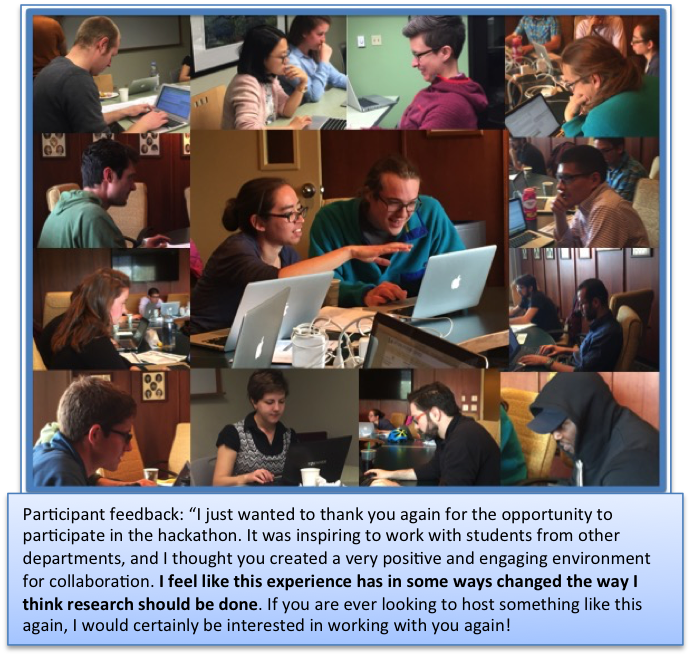
\includegraphics[width=0.5\textwidth]{figures/csu_hackathon.png}
\end{center}
\caption{\label{csu-r-hackathon} Some of the approximately 15 undergraduate students, graduate students, postdoctoral fellows, and professors who participated in a two-day Weather Data Hackathon at Colorado State University in April 2016.}
\end{figure}

\textbf{Long-term evaluation}:

\begin{itemize}
\item Google Analytics for online book. How often are people accessing the book? How long are they spending on the book website? Where are the people accessing the book?
\item YouTube analytics for the embedded videos. How often are people accessing the book? How long are they spending on the book website? Where are the people accessing the book?
\item Quiz for each chapter of the book? Use to evaluate how well they've mastered the material? (Possibly could use embedded Shiny apps for this? Other ways to do this?)
\item Rating options for each chapter of the online book? Usefulness? What they learned?
\item Survey within each chapter of the online book? Educational level, demographic characteristics.
\end{itemize}

\textbf{Things we want to know about the final training materials:}

\textit{Quantitative:}

\begin{itemize}
\item How many people have accessed the online book?
\item How are book users distributed across the U.S.? Are there many international users accessing the book?
\item When someone accesses the online book, how long on average do they spend reading or exploring the book? How many users are spending more than 10 minutes on the book per visit (about the minimum time for a module)?
\item How many people have downloaded the entire book?
\item How many people have commented on or made suggestions for the book through its ``Issues" page?
\item How many people have viewed each of the tutorial videos?
\item What percent of people who begin to watch each video finish it? 
\item For each video, are there common locations in the video where many people turn it off?
\item For online quizzes, how many people take each quiz?
\item For each quiz question, what percent of people answer it correctly? Are there some questions that many trainees struggle with after going through the training material?
\item For audio files of Co-Is answering discussion questions, how often do people listen to those? How many people listen to the complete file?
\item For applied exercise that include data or files to download, how many people have downloaded the files?
\item What is the demographic profile of users (age, gender, race, ...)?
\item What is the educational profile of users (highest degree, area of research)?
\item What is the professional profile of users (current position, typical research tasks for which the trainee is responsible)?
\item For each module, which elements did a trainee use (online book text, video tutorial, additional content like discussion questions and quizzes)? How useful did the trainee find each of the elements he or she used (on a Likert scale)?
\item For each module, did the user feel that he or she had adequate prior knowledge to follow the material in the module, or were there unstated prerequisites that the trainee lacked and felt limited their ability to learn from the training module?
\item For each module, does the trainee anticipate making any changes to his / her research practice based on having taken this module?
\item For each module, what percent of the material was new to the trainee (versus things he or she had already learned or heard about outside of the module)?
\end{itemize}

\textit{Qualitative:}

\begin{itemize}
\item What types of suggestions and comments have people made about the book through its ``Issues" page? Are these mostly to fix typos, or are there substantive questions? Have users helped to identify areas with which they struggled?
\item What are the users' goals in taking the training modules?
\item How did the user decide which modules to take?
\item For each module, what are elements that the trainee wished had been covered but were not?
\item For each module, were there elements that the trainee did not find useful that could have been excluded?
\item For each module, how did the trainee use any additional materials (discussion questions, quiz questions, applied exercises) that came with the module?
\item For each module, how does the trainee plan to change his or her research practice based on having taken the module?
\item Did the trainee consider using other training materials to learn this material (e.g., on-campus courses, online MOOCs, other books or video series)? If so, what aspects of our training materials led to the decision to pick them?
\item Why did the trainee decide to use these training modules (e.g., requirement for a course, PI told them to, self-motivated to improve their research practices, interested in learning new technology)?
\end{itemize}

\textbf{Levels of evaluation:}

\begin{itemize}
\item \textbf{Final users of the online book and videos.} These could potentially be from anywhere in the world, and for many we won't have great ways to contact them. 
\item \textbf{Workshop attendees for the workshops we plan to propose and do at national microbiology / immunology conferences.} For these people, we could definitely do a survey before to get information on demographics, education level, interest in the training materials, etc. We could also do a post survey to find out what they learned, how helpful it was, what they found confusing, etc. Finally, we could get their email addresses to ask some longer-term evaluation questions (e.g., How are they using what they learned 1--2 years after taking the workshop? How much did they retain in terms of principals, implementation, and examples?). We can also use questions that are asked during the workshops and areas where additional materials (applied exercises, quizzes, discussion questions) are problematic to help us hone our training materials.
\item \textbf{Early online users.} We will plan to develop and post the text and some of the additional educational materials (e.g., quizzes, discussion questions) online through GitHub \textit{as we write the book and develop the materials}. We will use social media to invite people to try out the book as we develop it. Based on previous work developing online books, we have found that this open development process can help attract users very early in the process, and that these users are often very helpful in providing feedback as the book is developed. We will elicit their feedback through GitHub (``Issues" page will be the main forum for them to post comments and suggestions).
\item \textbf{CSU pilot users.} We can ask these pilot users many questions, both before and after the pilot testing. Further, we will have access to ask them longer-term outcomes, as well as to ask at the department level how the use of these training materials by a number of people in the department has changed research practices and what is considered ``best practice" for research in the department (i.e., a `bubble up" effect).
\item \textbf{Pilot users from other institutions.} Similar to CSU pilot users, although we'll have a bit less access for determining longer-term and department-wide outcomes.
\end{itemize}

\subsection{Dissemination Plan}

\begin{quotation}
``A specific plan must be provided to disseminate the finished training modules \textbf{nationally} and make them \textbf{freely accessible}. In addition, links to these modules will be posted and maintained on the NIGMS web site."
\end{quotation}

We will create an online tutorial book, since providing tutorials, example code, and example datasets can substantially improve the ability of new users to learn software tools \cite{list2017ten}. We will use GitHub's free ``Pages" web publishing framework to publish the book freely online, and we will also submit it to the \textit{bookdown.org} website under a Creative Commons license. Dr. Anderson (PI) has previously created two \textit{bookdown}-based books, \textit{R Programming for Research} and \textit{Mastering Software Development in R}. Both are publicly and freely available online under the Creative Commons license (see LOS, Xie). 

We will publish the video lectures using the YouTube platform and embed these videos within the online book. The videos, like the book, will be published under a Creative Commons license.

For many online training materials on the principals and implementation of computationally reproducible research, the target audience is statisticians and other researchers who focus on data analysis. This audience now has access to many excellent resources for improving research reproducibility at the data analysis stage. Our target audience is instead researchers who focus on conducting experimental, laboratory-based biomedical research and whose research tasks are more focused on the earlier research steps of running experiments, recording experimental data, and pre-processing that data, prior to data analysis steps. We are focusing our dissemination plans on this target audience, for whom training materials on improving the reproducibility of later data analysis steps might be of limited relevance.

We will also take steps to make sure that our target audience---laboratory-based biomedical scientists---are aware of these training materials. We will travel in Years 02 and 03 to one national microbiology ([conference]) and one national immunology ([conference]) conference. We will submit proposals to these conferences to present half-day (student?) workshops covering why and how to improve reproducibility in experimental data recording and pre-processing for biomedical microbiology and immunology research. We will also submit poster abstracts to present and discuss the training materials as part of each conference's poster sessions. We have budgeted for two members of our team (the PI and one co-I) to attend each of these conferences to help disseminate the training materials produced by the project. [CSU's microbiology seminar series? Conferences on-campus at CSU? Are there ones that are repeated every year?]

The PI has previously had substantial success in disseminating online training materials. She is the co-instructor of a five-course specialization on \textit{Mastering Software Development in R} through the Massive Open Online Course platform Coursera. The first course in this series has had over 25,000 participants since it was opened in fall 2016. An accompanying online book on the LeanPub platform has been accessed by [x] people. The PI, however, does not have a presence in the microbiology and immunology community, and so the co-investigators, who are heavily involved in this community, will form a key bridge in making sure our target audience is aware that these training materials are available.
    
\subsection{Timeline}

\begin{quotation}
``Provide a timeline for \textbf{module development}, \textbf{piloting and refinement}, \textbf{dissemination}, \textbf{evaluation}, and \textbf{maintenance}.  This timeline must propose making the training publicly available within two years of the award date."
\end{quotation}


\clearpage

\section{Works cited}

\bibliographystyle{unsrtnat}
\bibliography{rep_modules}

\end{document}